%_____________________________________________________________________________________________ 
% LATEX Template: Department of Comp/IT BTech Project Reports
% Sample Chapter
% Sun Mar 27 10:25:35 IST 2011
%
% Note: Itemization, enumeration and other things not shown. A sample figure is included.
%_____________________________________________________________________________________________ 

{\let\clearpage\relax \chapter{Results and Discussion}}

We trained ARU Net on historical data, as done by the authors in the paper as well as on custom document data generated by us.After training ARU Net for 100 epochs just on the historical data with no augmentation, we get a base model which performs good on simple documents without any augmentation but misses out the lines in the documents which are randomly oriented and have noise.After 100 epochs, the average loss came to be around 0.05438. This was done to reach to the level of the baseline model provided by the authors. Then after adding augmentations and training on the mixed set of data from IAM, some proprietary images and historic documents, it became robust on all sorts of images agnostic of noise,distortions etc. After 200 epochs, the average validation loss came to be around 0.07226.Further training of the model, decreases the loss but the effect on the baselines produced is not so considerable in terms of final post-processed outputs we achieve and it saturates after around 110 epochs, the model with best results is also obtained on 110th epoch.The graphs attached here are for training on custom data.

Although the ARU Net can work on images of any size, we found out that keeping the size fixed (768x768px in our case)  gives better results.We also trained just U-Net, R-UNet(with residual connections) and AR-UNet(with residual connections and Attention) separately and found out that ARU Net works best to capture better representations and to reach at better baselines.

As far as inference results are concerned, the trained model does a descent job on prediction of baselines in most of the cases of machine print but the post processing results using connected component analysis are not accurate in all the cases, we get two boxes for a word/line sometimes and sometimes the word boxes spread to the line below, leading to inaccurate character recognitions in the subsequent steps.Some of the results are attached here with.For handwritten documents which already have lines under the text(lines present in notebook), the baseline predictions are not good enough in those cases.

{\Large  \textbf{ARU Net: Graphs}}

\begin{figure}[H]
	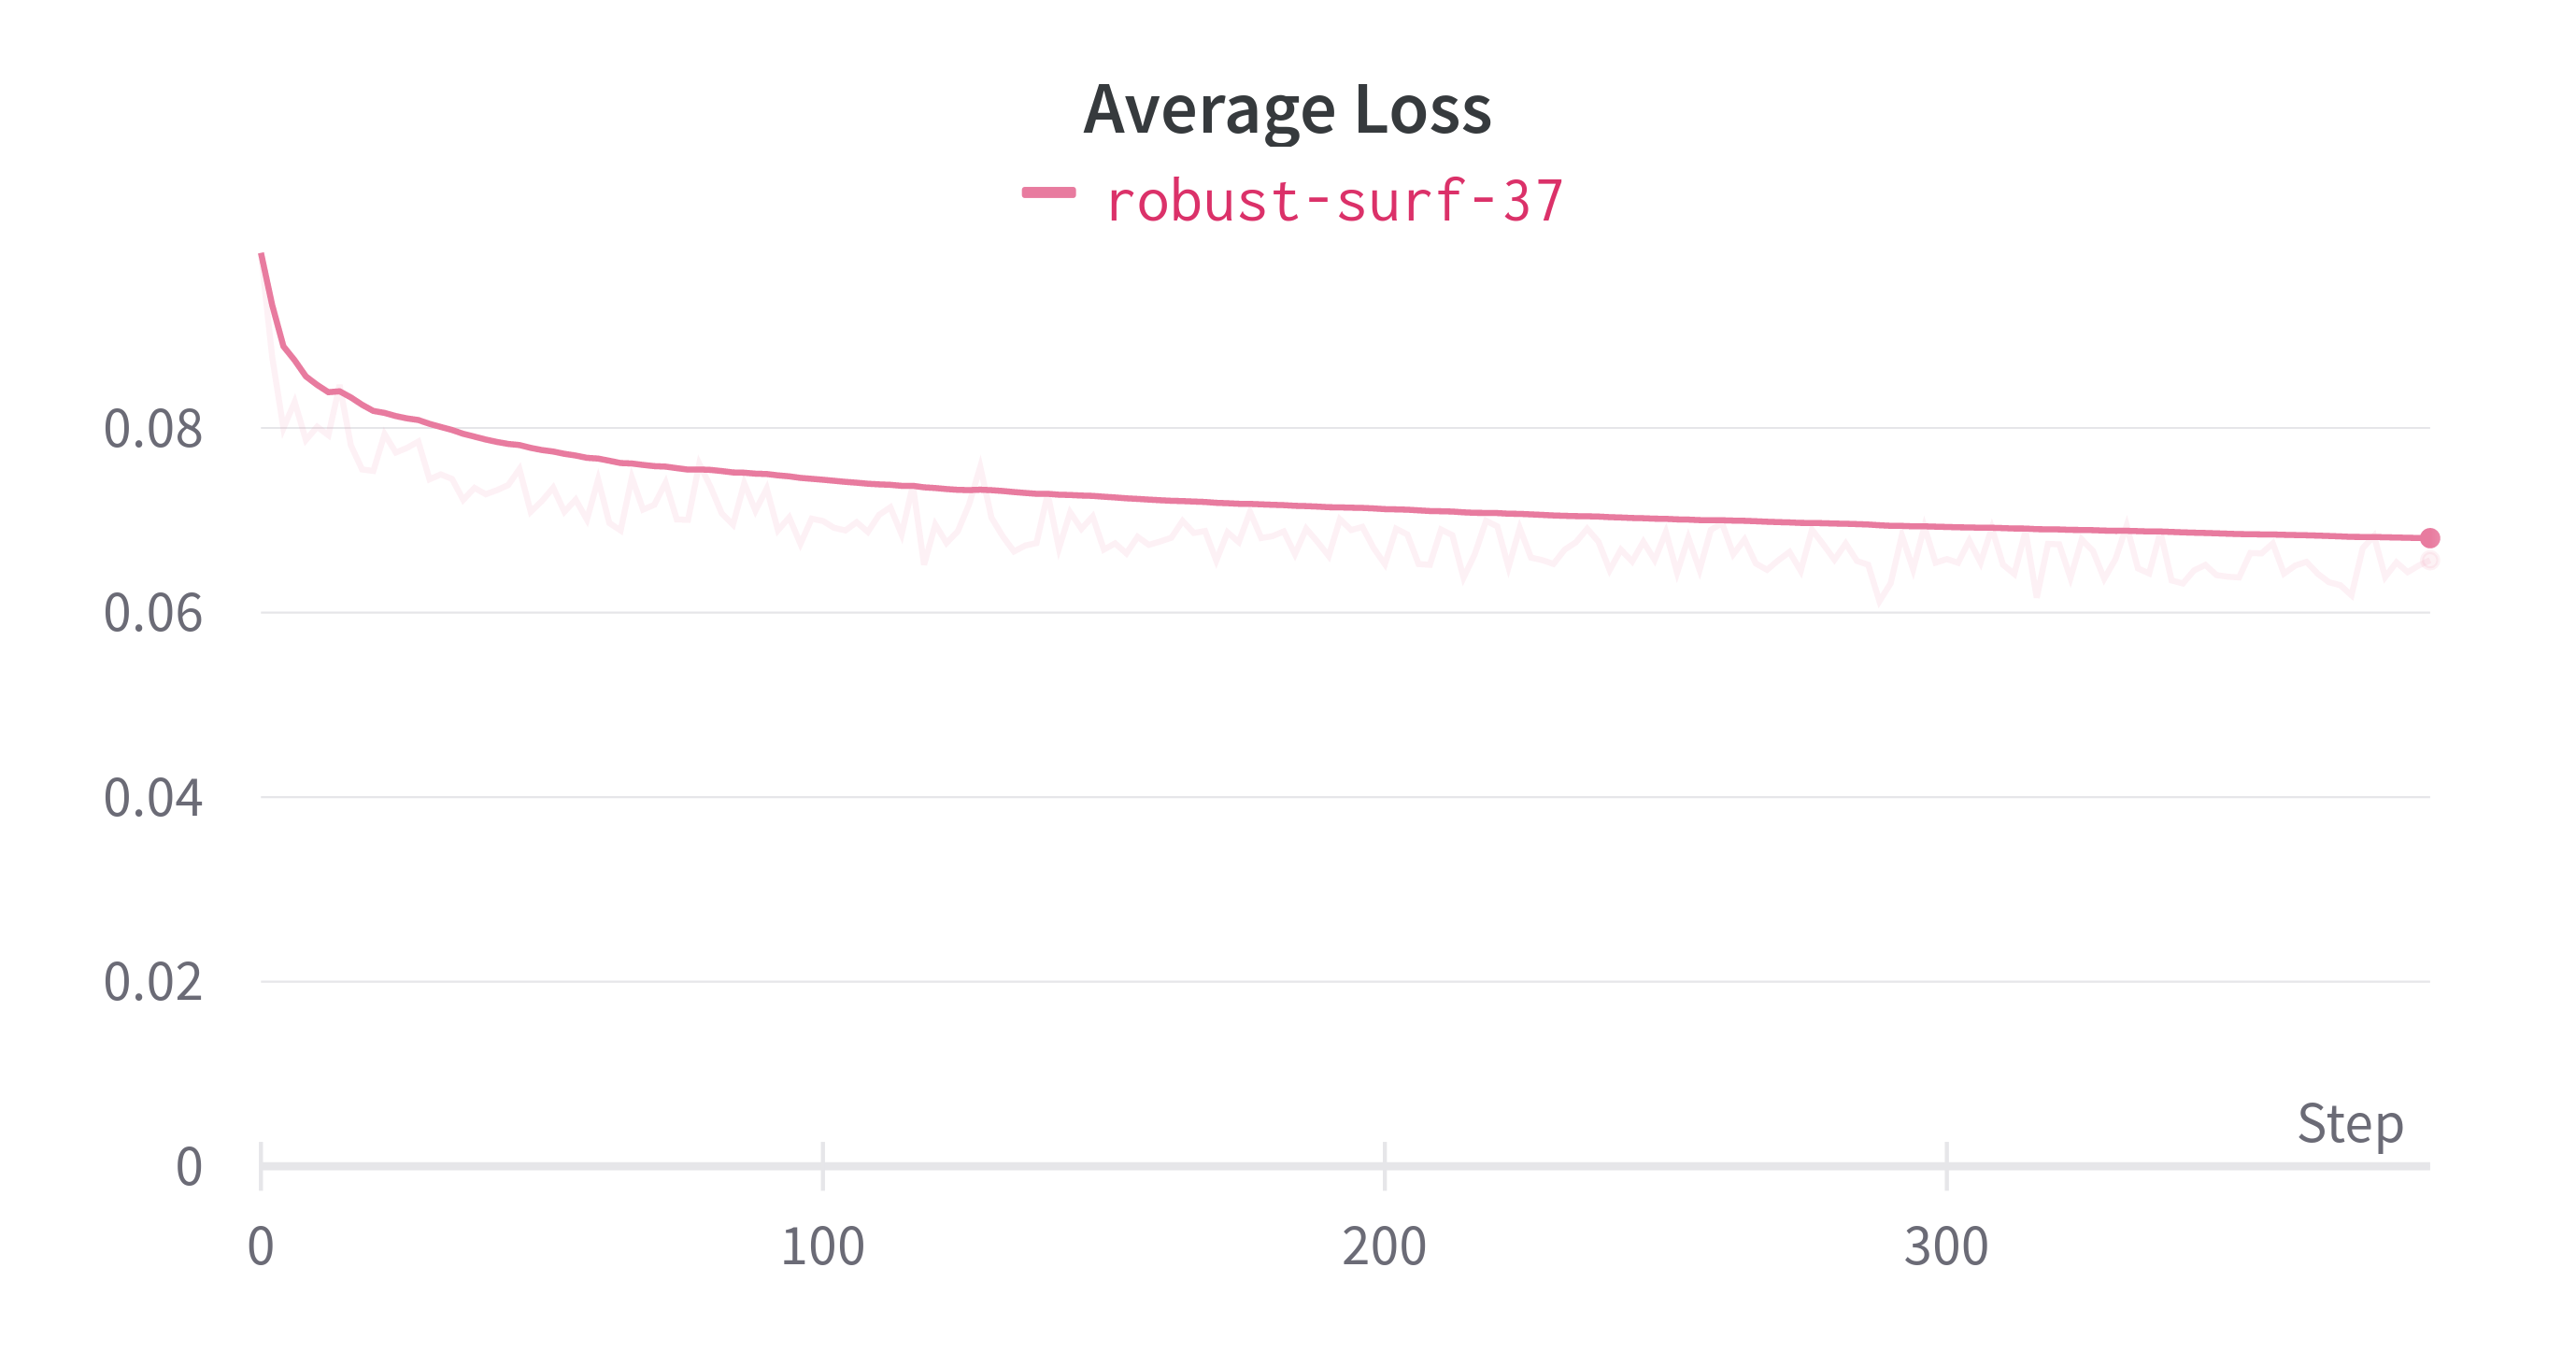
\includegraphics[width=475pt,height=275pt]{Training Loss ARU Net.png}
	\caption{Average Training Loss: ARU Net}
\end{figure}

\begin{figure}[H]
	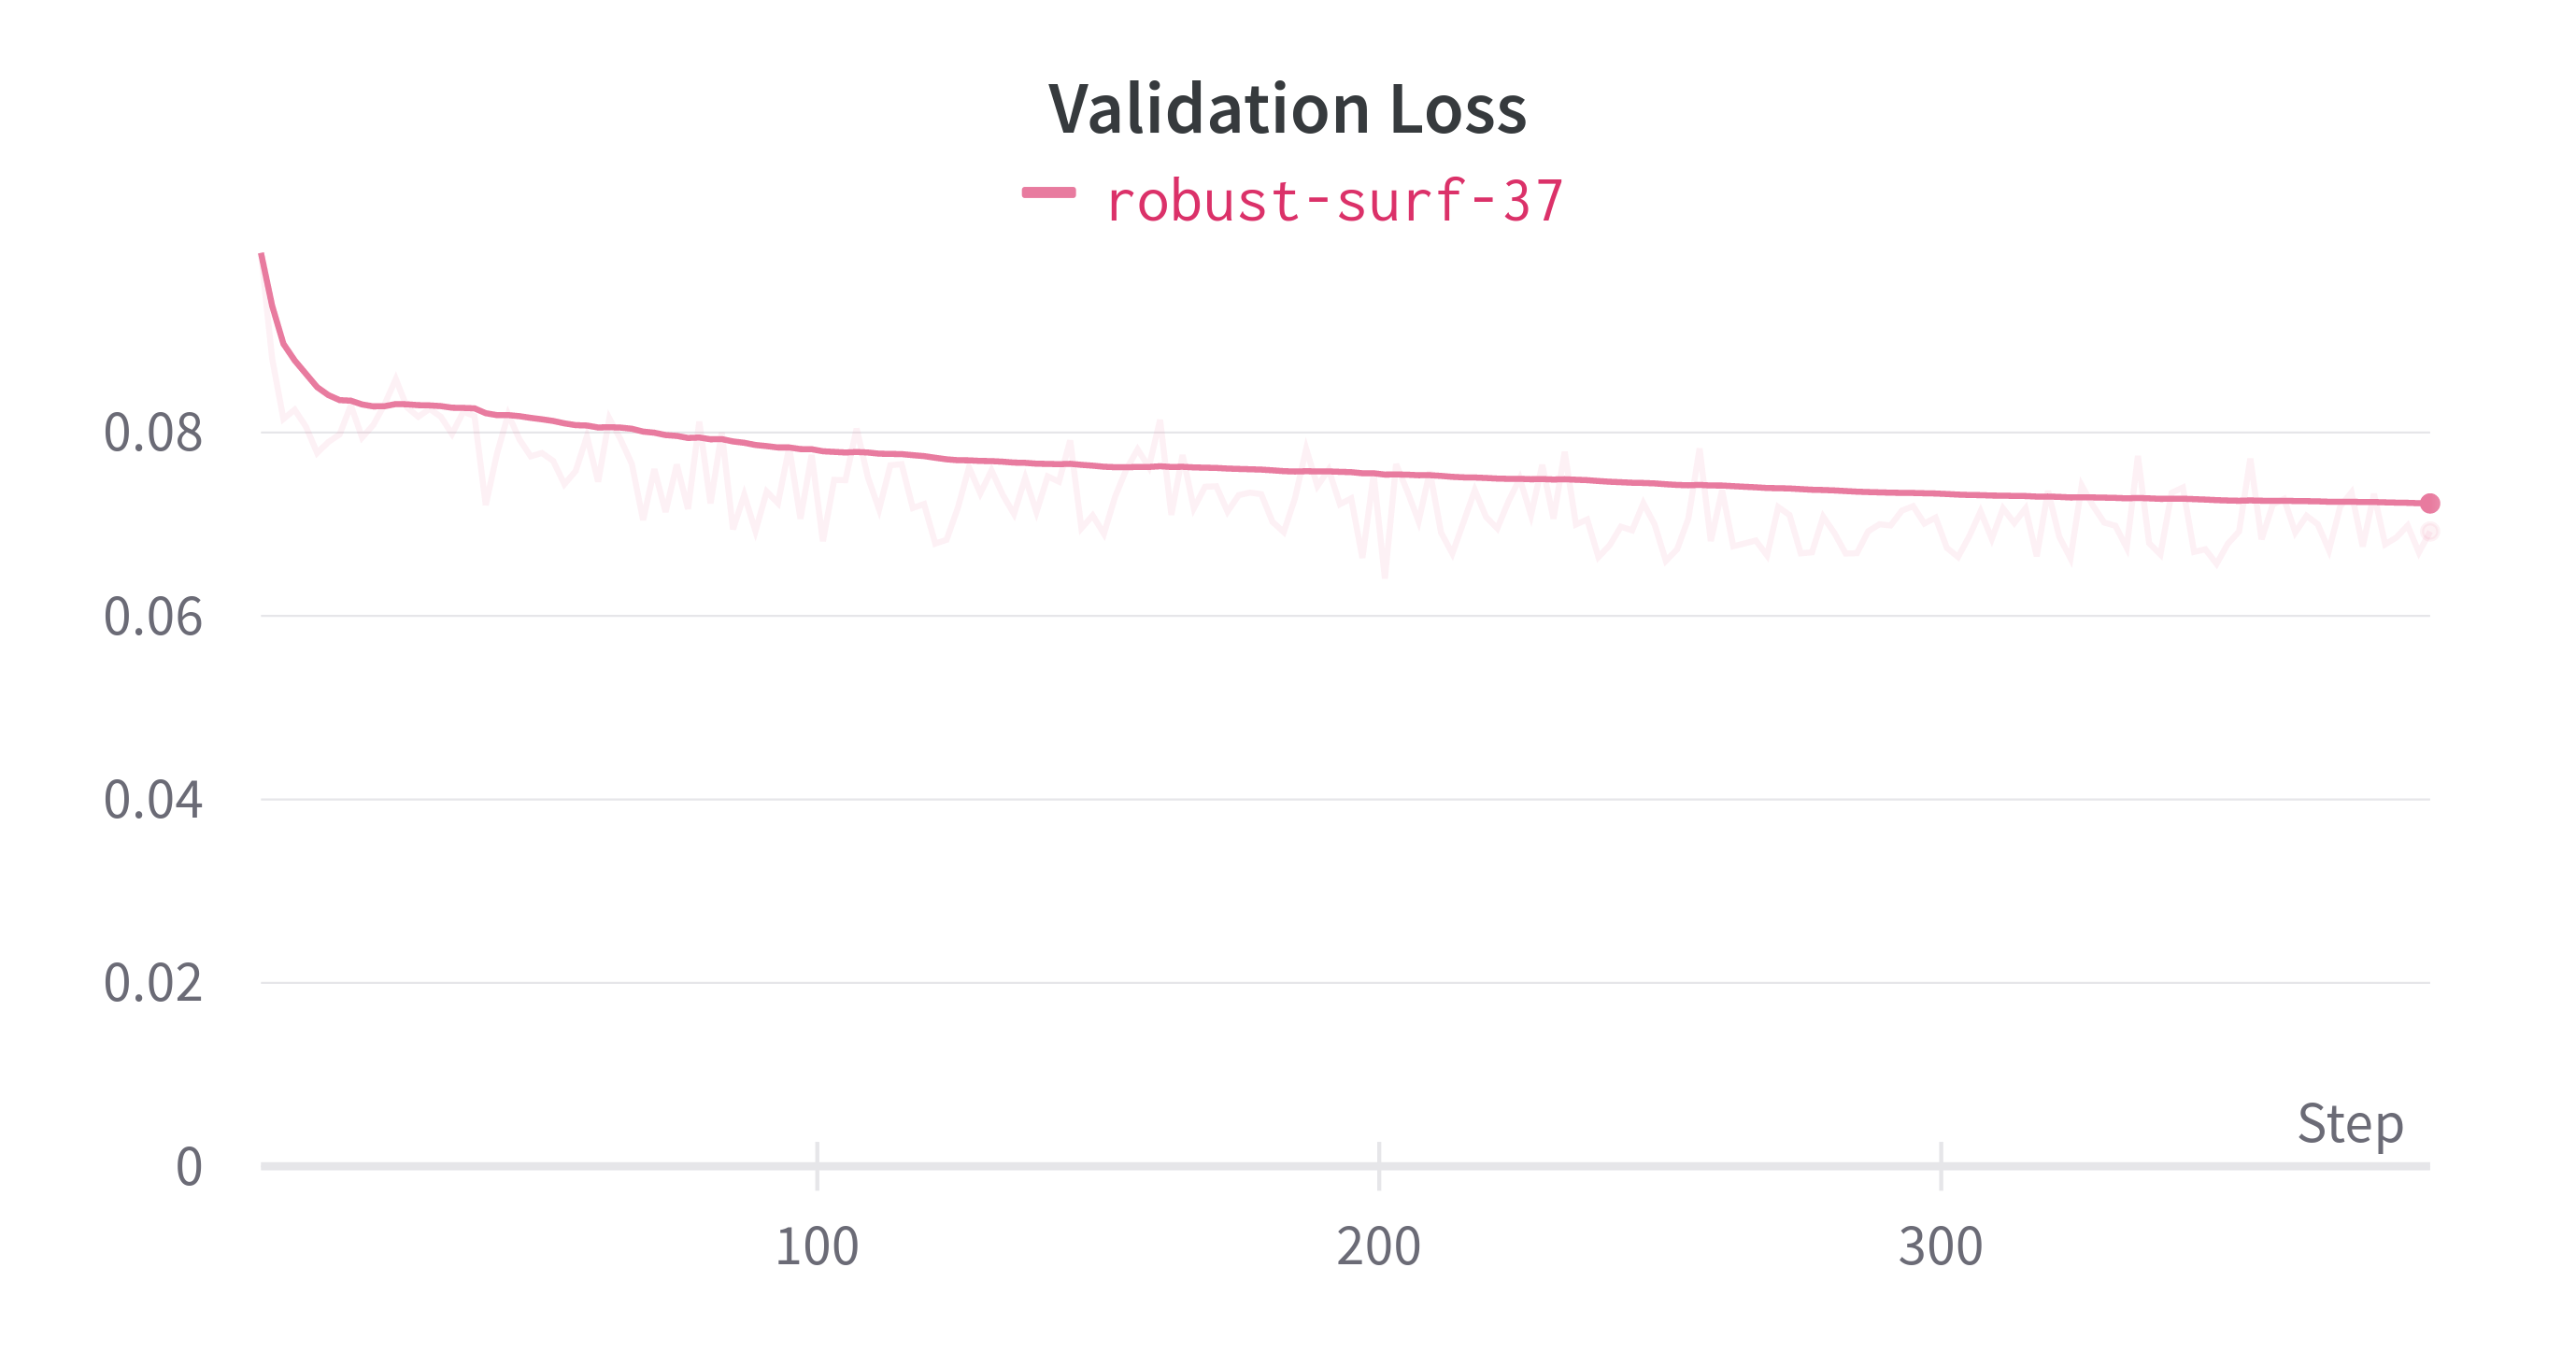
\includegraphics[width=475pt,height=275pt]{Validation Loss ARU Net.png}
	\caption{Validation Loss: ARU Net}
\end{figure}

\begin{figure}[H]
	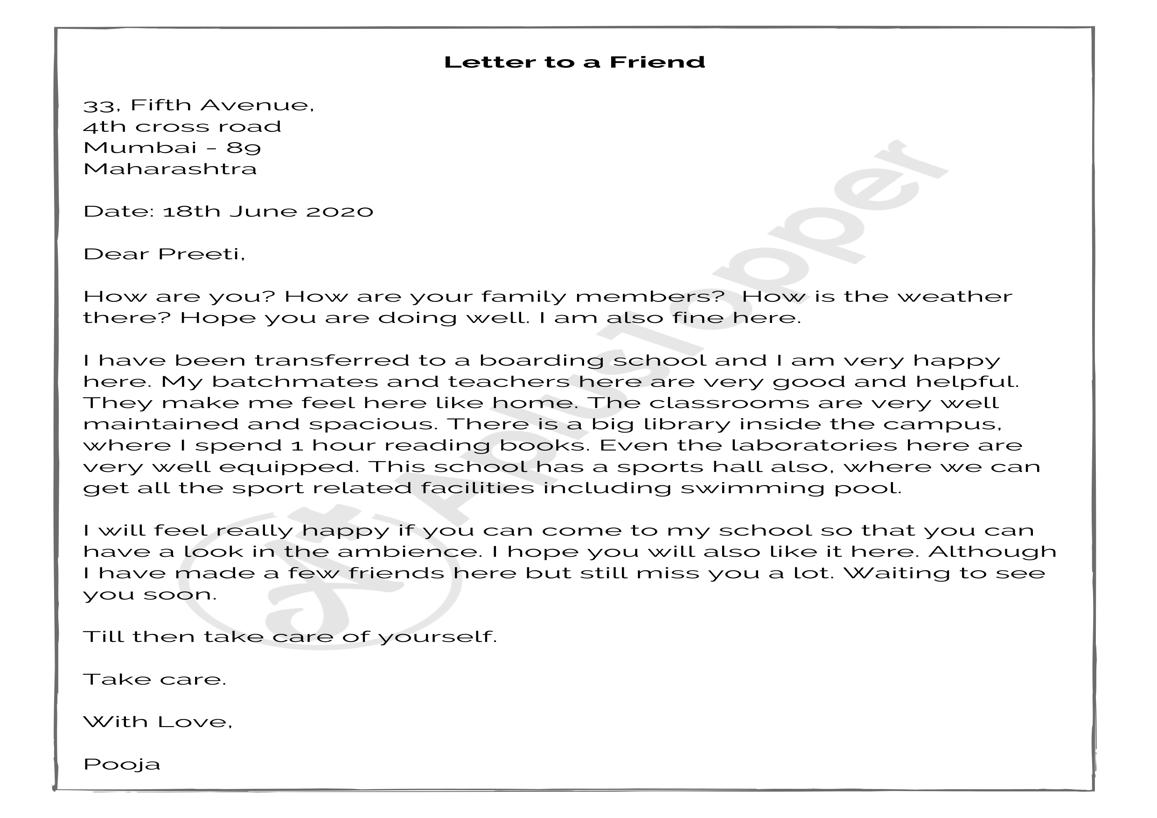
\includegraphics[width=475pt,height=275pt]{in.jpg}
	\caption{Input: ARU Net}
\end{figure}

\begin{figure}[H]
	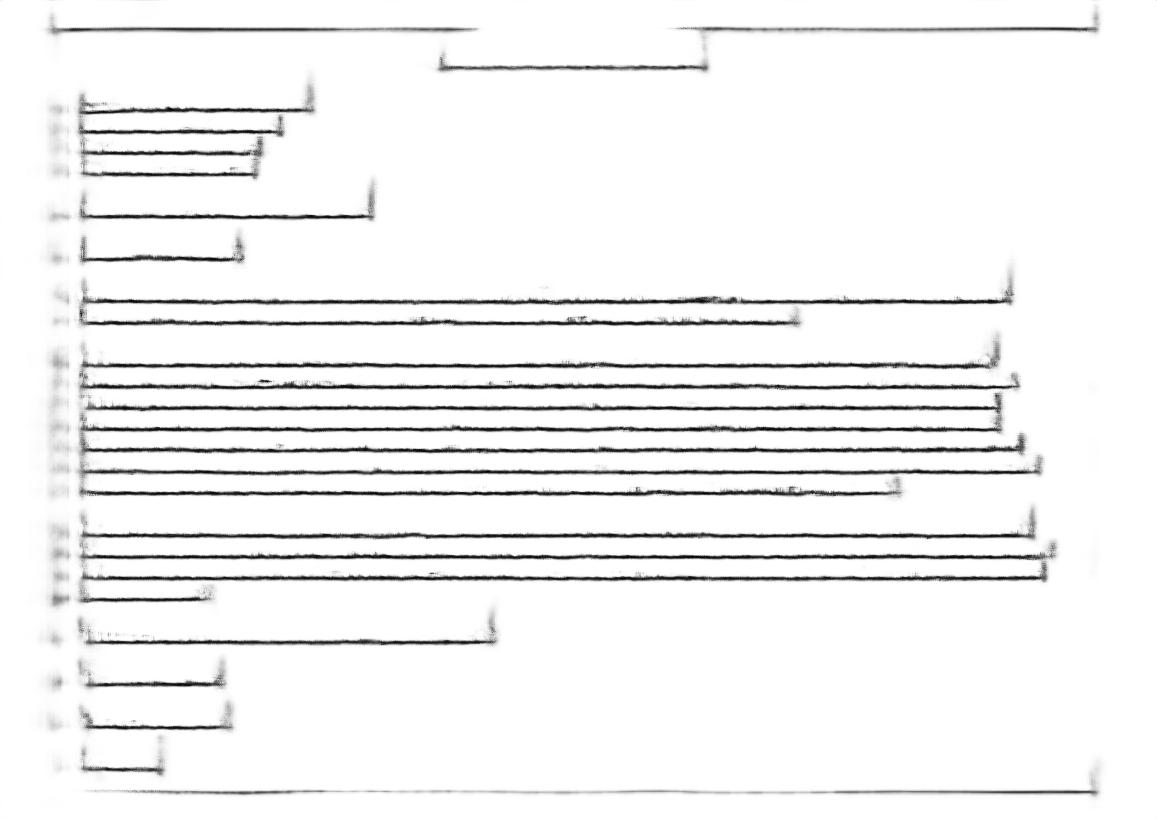
\includegraphics[width=475pt,height=275pt]{out.jpg}
	\caption{Output: ARU Net}
\end{figure}


\begin{figure}[H]
	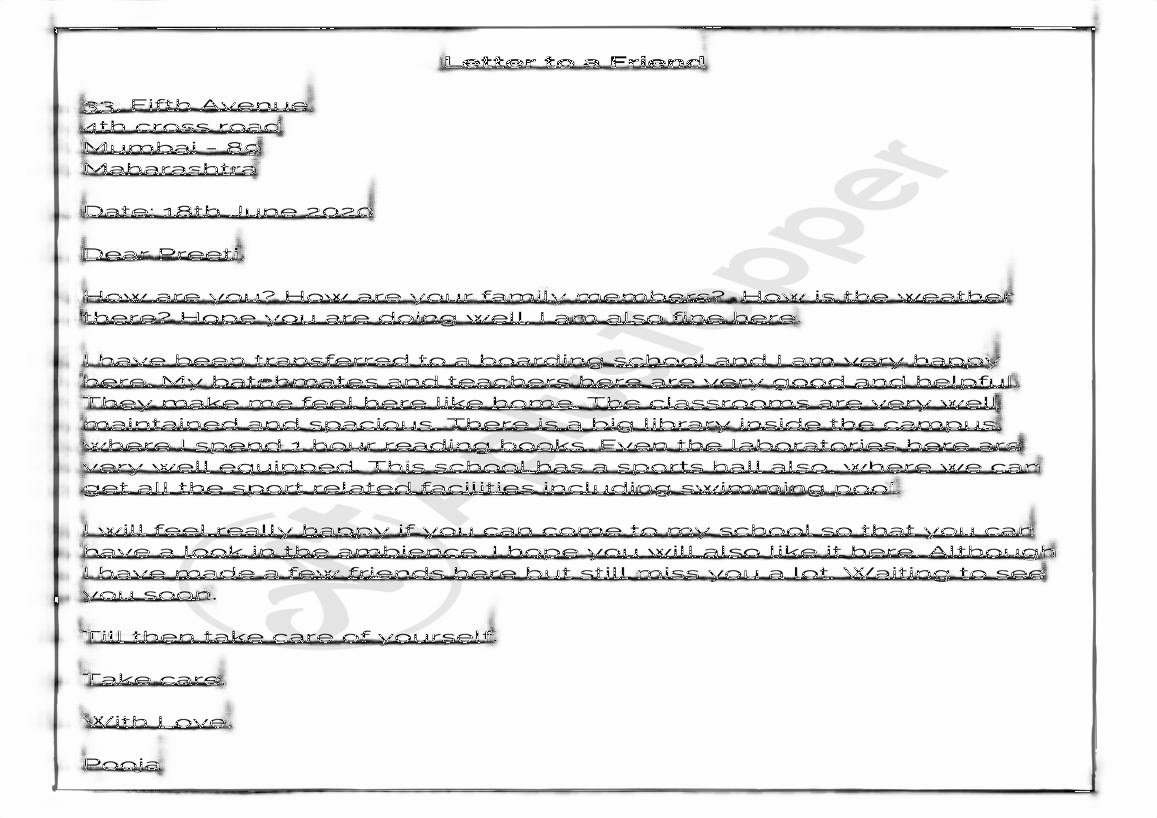
\includegraphics[width=475pt,height=275pt]{res.jpg}
	\caption{Intermediate Result: ARU Net}
\end{figure}


\begin{figure}[H]
	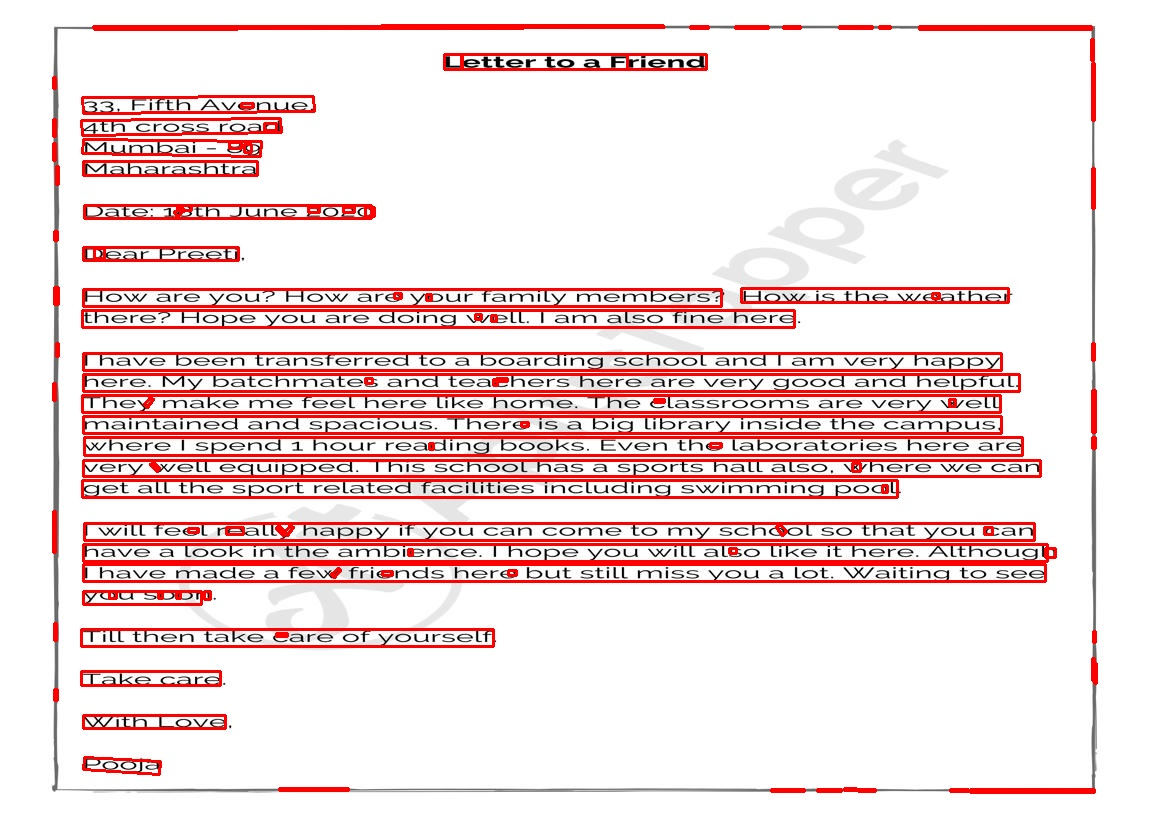
\includegraphics[width=475pt,height=275pt]{res_boxes.jpg}
	\caption{Bounding boxes: ARU Net}
\end{figure}

Shifting discussion to CRAFT network, the baseline model we started fine-tuning with, was trained on just synthetic data.Synthetic data was very different than document data where we have hundreds of words in a page as compared to just a few words in synthetic data.Also the size of the words is comparatively small as compared to synthetic dataset.The baseline model was not able to perform good on augmented documents in which text is at random angles.In all, the performance on the document data was not so great.We trained our model for around 100 epochs. An epoch takes around 90-100 minutes to complete and we analysed the results after every epoch. After certain epochs, the results start to degrade rather than improving,this can be due to the reason that the character level bounding boxes in the training data were not accurate and we were doing fully supervised learning of CRAFT.

In the first run, we didn't combine the input data with synthetic data as used by the authors and as a result, the network started to forget the past learned information and performed bad even on the examples the baseline model performed good, although the results on the handwritten documents improved a bit.

In second phase, in every batch, we combined our custom training data with synthetic data used for training the baseline model we started with,used in the ratio of 3:1 in every batch. The results of training the network with this change helped to stay good on the cases where baseline performs good as well as get better at handwritten text. There are still some issues in recognising the text in the handwritten documents in which ruling lines are present in the paper, for which the model fails to recognise the words.But the results of recognising the words on plain paper are quite good.Certain issues also exist in machine print documents where the CRAFT model fails to recognise small characters like comma,hyphens,points,single characters and it becomes extremely critical in certain business documents.The sample result images are attached here with. 

We also tuned the hyper parameters required for connected component analysis and obtaining words from region and affinity scores - link threshold, region threshold and text threshold. Region threshold filters out the pixels regions below certain value and link threshold does that for affinity scores. After combining region and affinity scores, we do connected component analysis and find a large number of components and then we use text threshold to select the appropriate components for finding the minimum area rectangles.

We have deployed the best epoch model which feeds in Word OCR model with the bounding boxes of all the words present in the page.The API is being used internally for testing. 

{\Large  \textbf{CRAFT: Graphs}}

\begin{figure}[H]
	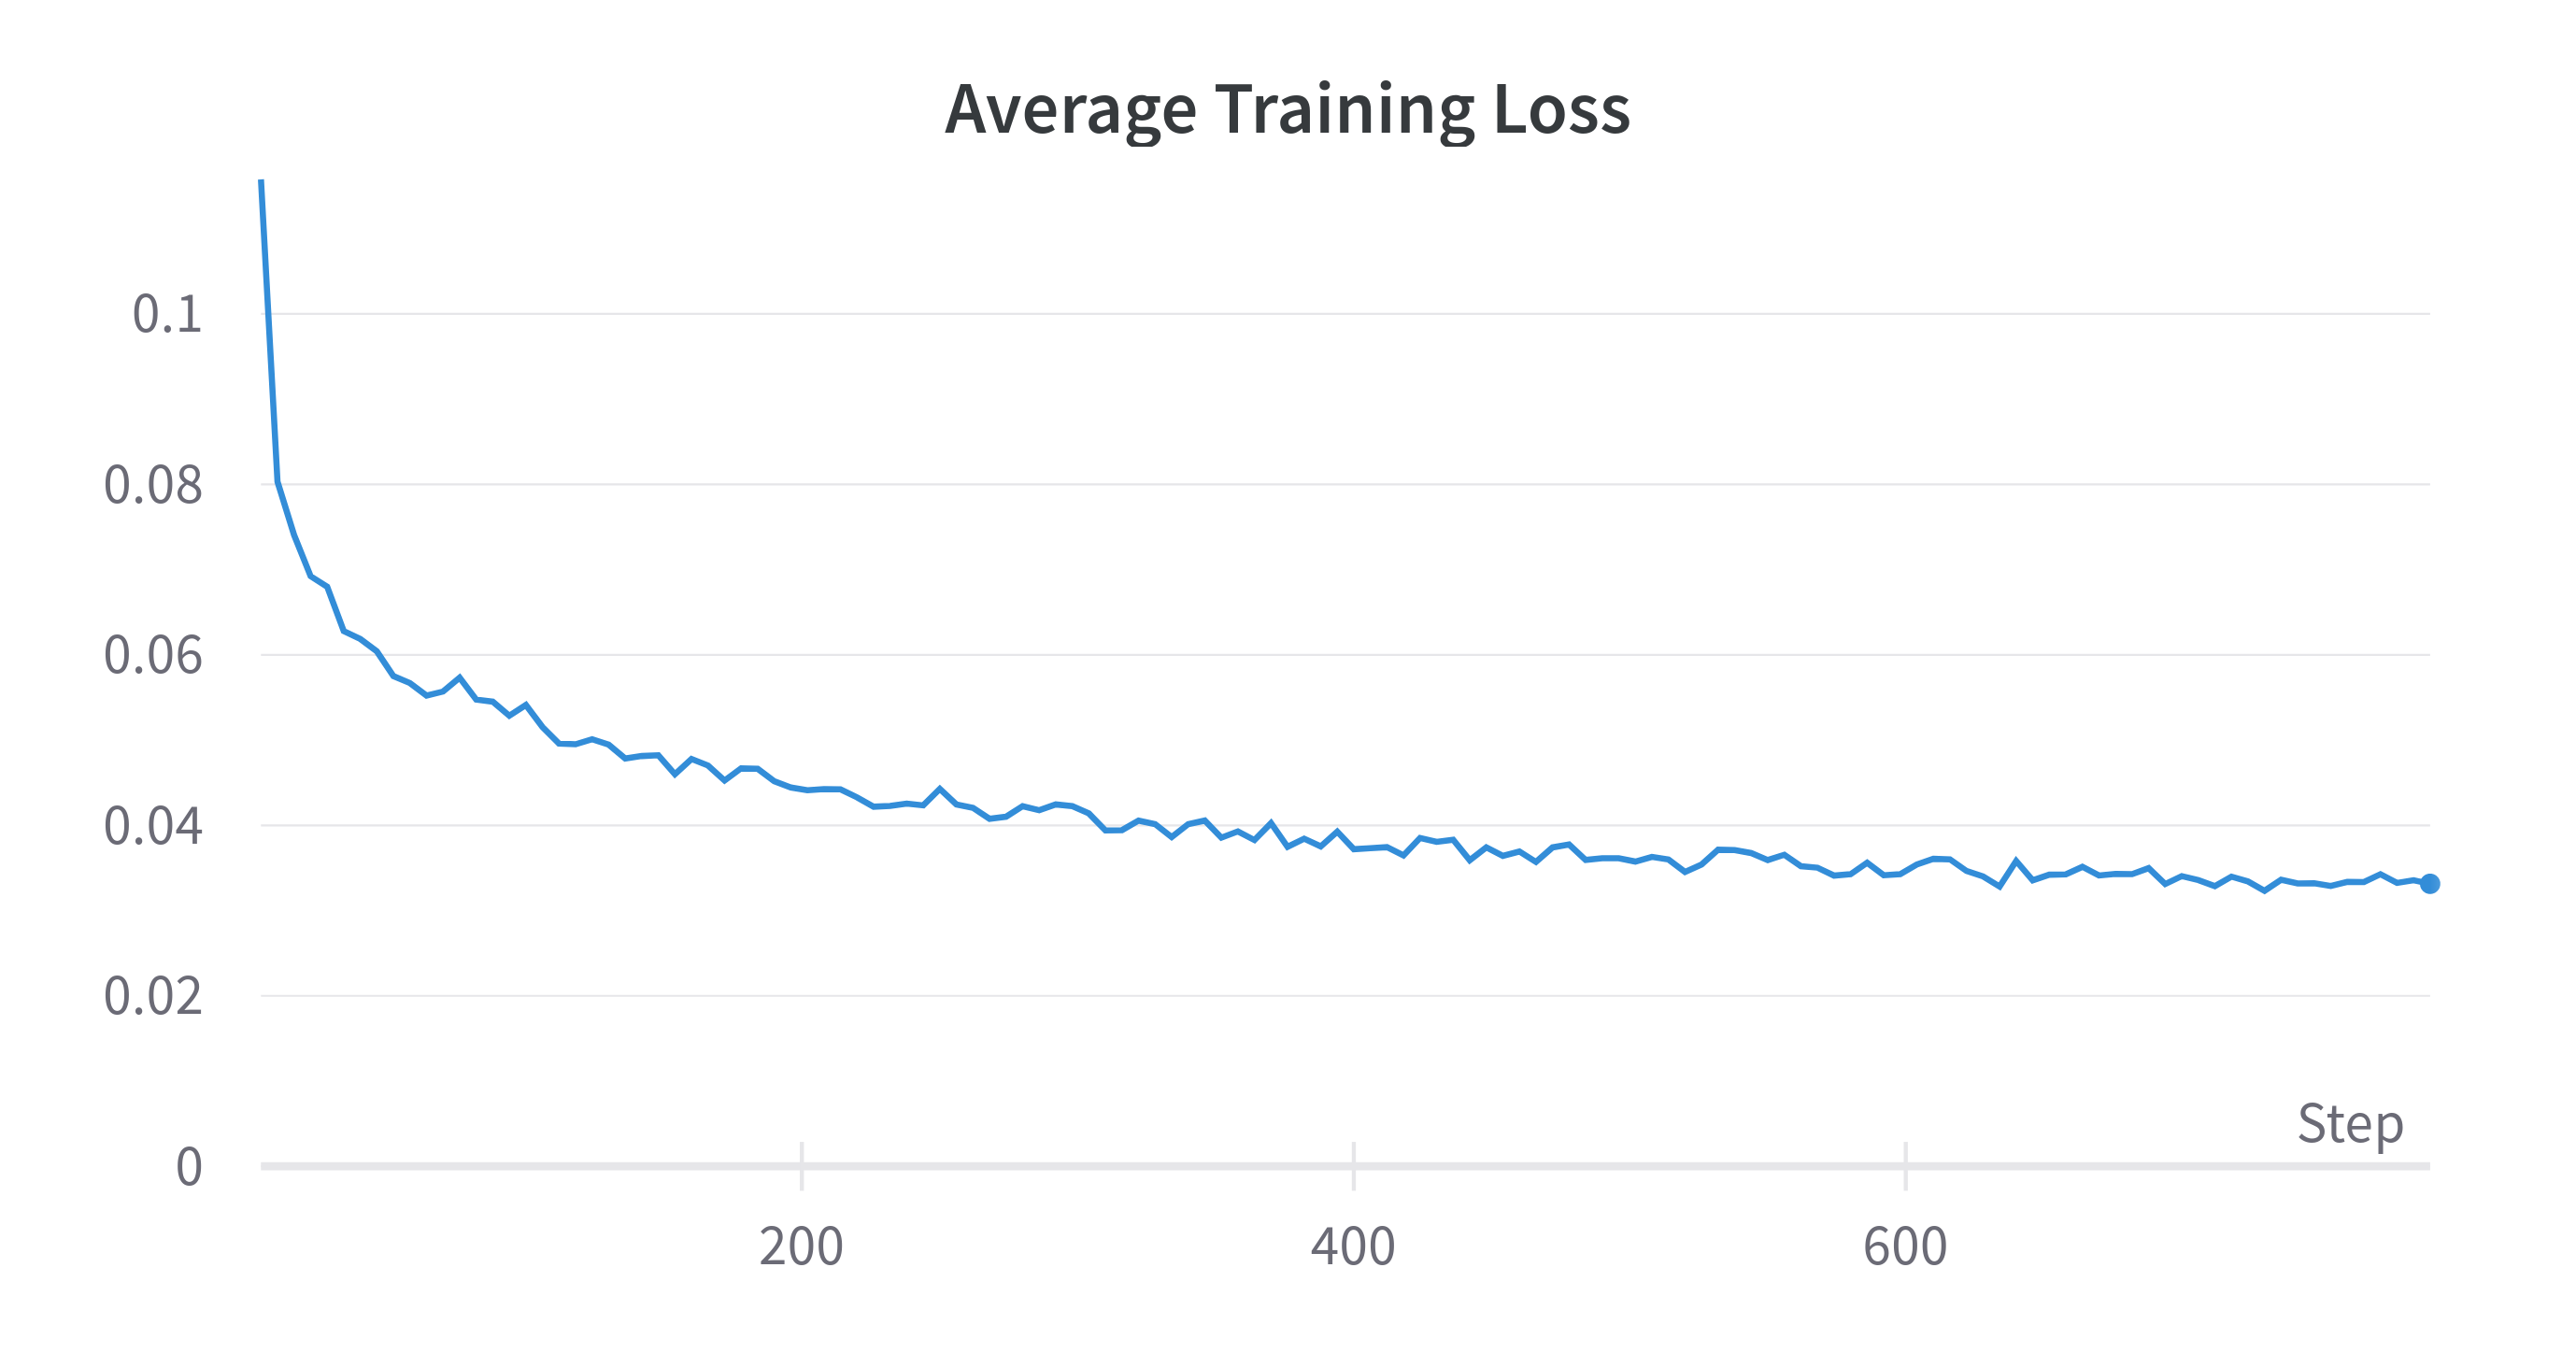
\includegraphics[width=475pt,height=275pt]{Training Loss CRAFT.png}
	\caption{Average Training Loss: CRAFT}
\end{figure}

\begin{figure}[H]
	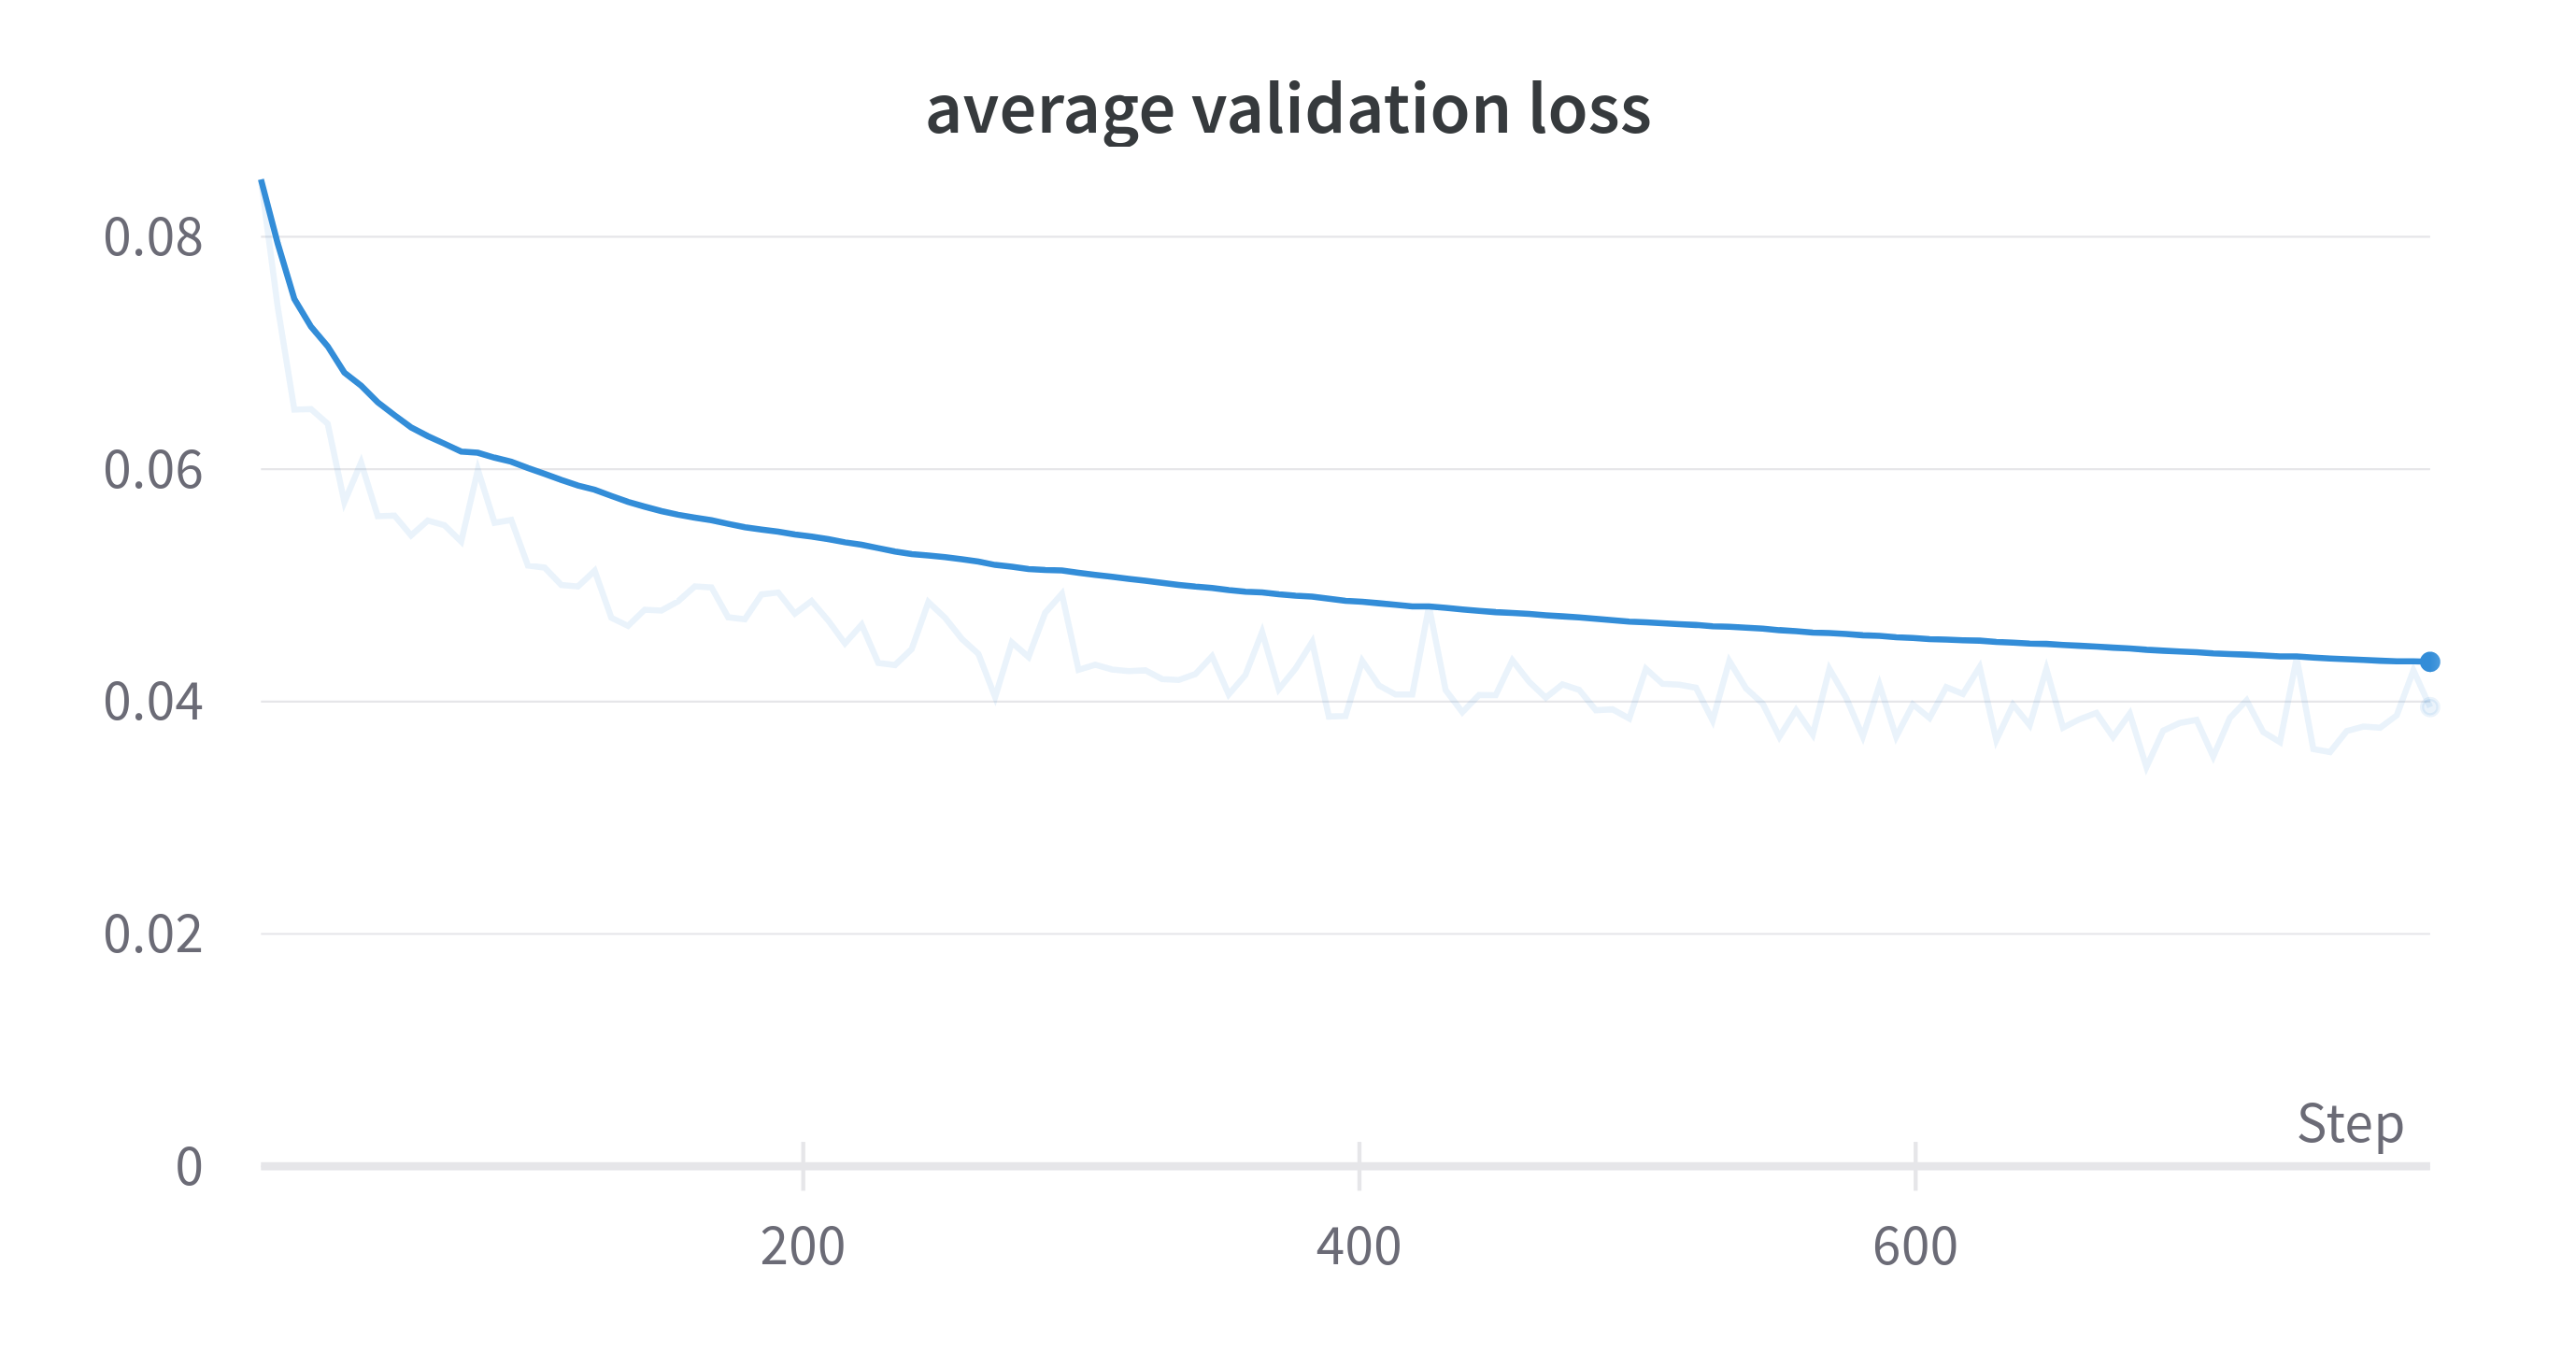
\includegraphics[width=475pt,height=275pt]{Validation Loss CRAFT.png}
	\caption{Validation Loss: CRAFT}
\end{figure}


\begin{figure}[H]
	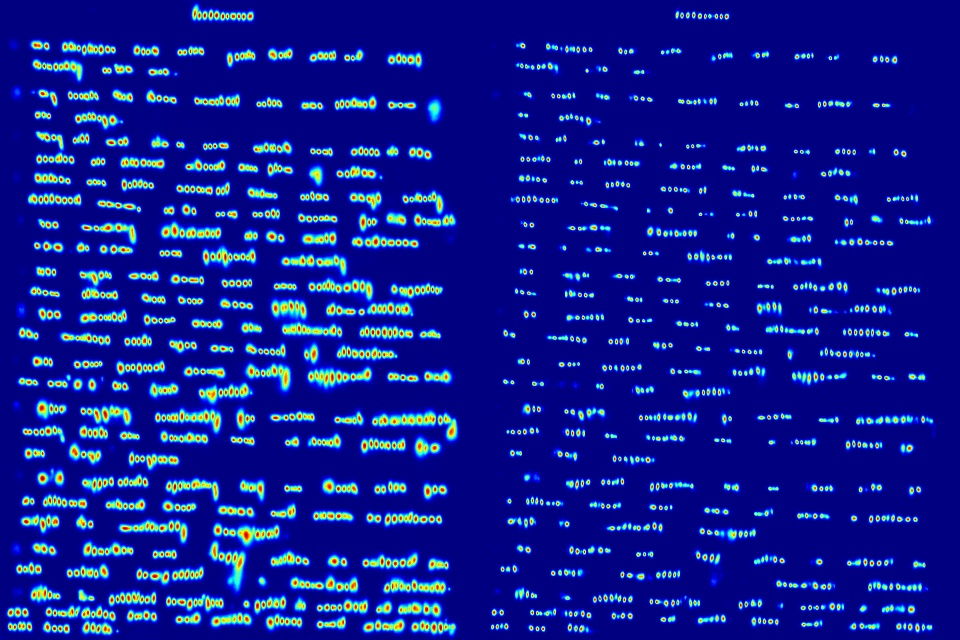
\includegraphics[width=475pt,height=275pt]{craft_mask.jpg}
	\caption{Masked output: CRAFT}
\end{figure}

\begin{figure}[H]
	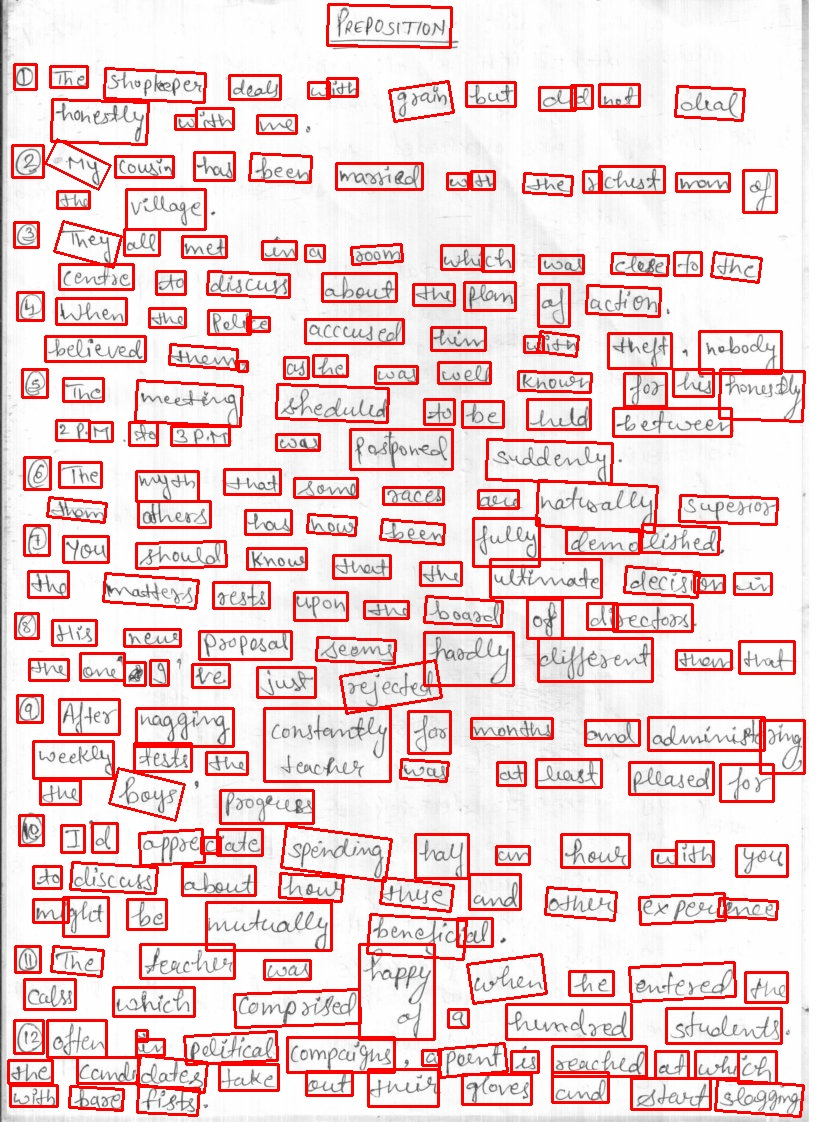
\includegraphics[width=475pt,height=275pt]{craft_out.jpg}
	\caption{Bounding Boxes: CRAFT}
\end{figure}

After introduction of word region maps, we were able to tackle the problems of word-splitting, detect missing symbols and handwritten words to a great extent.In the first iteration where we copied and opened up only last 5 convolutional layers for producing word score regions, the regions obtained did not match or even resemble the corresponding ground truth word regions that well. In the second modification,we copied the up-convolutional layers and the final convolutional layers, keeping the original up-convolutional layers frozen for computing region and affinity scores.After training the network with second modification, we were able to get a lot better word regions, looking visually very similar to the ground truth word scores.The visually improved word regions and the use of word region maps for arriving at final bounding boxes along with region and affinity maps also led to reduction in words splitting to a great extent, especially in the machine print documents.

In the post processing steps,we combined word scores with region and affinity scores and tuned various hyper parameters for obtaining word bounding boxes after doing connected component analysis.With hyper parameter adjustments, a significant improvement was also seen in detection of handwritten words.In some cases,we get no region and affinity scores but only word score regions for words in handwritten text and still we are able to detect the words after super-imposing all 3 score maps( character regions, affinity and word regions) before going through the connected component analysis followed by other post processing steps with appropriate region,affinity,word and text thresholds.For our use case, we selected text threshold as 0.3, link threshold as 0.3,region threshold as 0.4 and word threshold as 0.5.

\begin{figure}[H]
	\includegraphics[width=475pt,height=275pt]{res_image_63.jpg}
	\caption{Bounding Boxes: CRAFT on IAM image}
\end{figure}

\begin{figure}[H]
	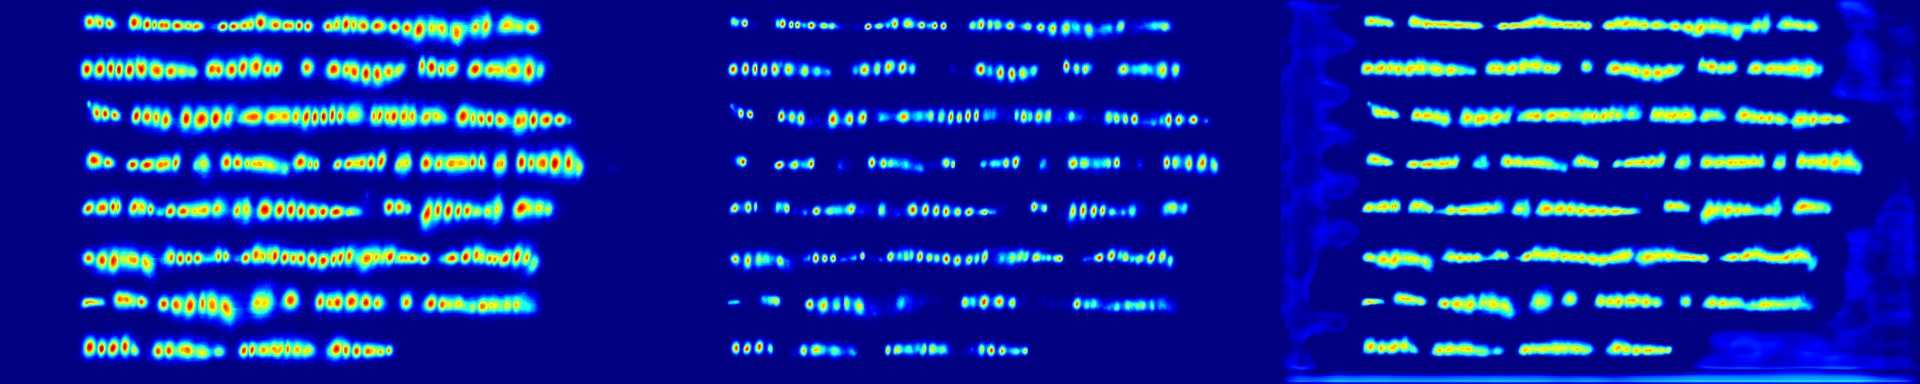
\includegraphics[width=500pt,height=235pt]{res_image_63_mask.jpg}
	\caption{Masked output: CRAFT with word scores}
\end{figure}

We prepared a custom precision and recall metric based on Intersection Over Union of detected word bounding boxes and the ground truth word boxes and used that for evaluation over a set of test images. The metric considers a detected word box as correct prediction if the IOU with the ground truth box exceeds a certain threshold. We evaluated the test set with the metric over various thresholds to know the corresponding precision and recall.


%_____________________________________________________________________________________________ 
